\chapter{Introduction}
\label{ch:introduction}

Robotic manipulation of objects is an increasing field of research which has struggled researches from many years ago. In several industrial environments robots can be easily programmed considering the objects to be known a priori, i.e. the manipulation is always the same, and usually robot operations avoid to deal in cluttered scene, but this situation needs a workspace designed in a manner to provide to the robot a non cluttered scene. But there are situations in which robots with enhanced intelligence can be useful.
 An example in which a robot could face a cluttered scenario is the one of the \textit{Amazon Picking Challenge} \citep{APC}, which has the objective to provide a challenge problem to the robotics research community that involves integrating the state of the art in object perception, motion planning, grasp planning, and task planning to manipulate real-world items in industrial settings such ones human operators face in Amazon's warehouse. Joey Durham from Amazon Robotics describes the challenges of this competition with the following sentence:
\begin{displayquote}
 “A robot for picking purposes must possess a lot of skills: The selected item must be identified, handled and deposited correctly and safely. This requires a certain level of visual, tactile and haptic perceptive skills and great handling capabilities.”
\end{displayquote}

In this thesis we are going to investigate a simple approach for a complex manipulation problem. Our approach tries to replicate the human reasoning during the manipulation of cluttered objects in table clearing tasks. The objective is removing all the objects onto a table considering that their poses could limit the manipulation actions. 

This thesis has been developed in the \textbf{Institut de Robòtica i Informàtica Industrial} (IRI) in the  Perception and Manipulation laboratory with the supervision of \textit{Guillem Alenyá Ribas} as director and \textit{David Martinéz Martinéz} as co-director. 

\iffalse
This chapter is structured as follow, first an introduction to the problem and the approach used is commented, then a review of the state of the art regarding manipulation planning is presented to the reader and final the experimental set up is presented since it will be useful to understand some techniques and choice for the algorithm which will be discussed in the next chapters. 
\fi

This work is structured as follow. First an introduction to the problem we want to solve is presented in the Chapter \ref{ch:introduction}. Then in Chapter \ref{ch:state_of_the_art} a review of the current state of the art in manipulation planning is done. The planner developed will be commented in Chapter \ref{ch:task_planner} and the implemented algorithm to compute the predicates and control the robot will be commented in Chapter \ref{ch:algorithm}. In Chapter \ref{ch:implementation} the softwares employed for the implementation of the code will be presented as well the algorithm's structure. Finally some experiments and conclusions about this work are discussed in Chapter \ref{ch:experiments} and \ref{ch:conclusions} respectively.

In this chapter first an introduction to the problem and the approach adopted is commented, then the experimental set up is presented since it will be useful to understand some techniques and choices for the algorithm which will be discussed in next chapters. 

\section{Problem Approach}
In this section the approach to solve the planning problem is described. The strategy to solve the problem is inspired to a human-like solution. A human would solve such task with three main actions: grasp an object, push it or drag it. When it is not possible to grasp an object, because other objects hinder the human to put the hands in the proper way to grasp the desired one, he/she has to interact with the scene in order to put the desired object in a pose where it can be grasped.

Dragging is a very complex action which will require the robot to lay the end effector on the top of an object. This is a very hard action which would imply an implementation of a reliable controller, moreover the goal is not only to move the object but also not to ruin it.

Pushing action is an action easier than dragging since it only requires to put the end effector in a certain pose and then push the object by moving the end effector. However the pushing action is complex since to push an object making it following a certain path the pushing pose has to be chosen taking into account the shape of the object and a controller would be needed in order to correct the pose along the path. Despite this we handled to perform that action in a easy way by considering only objects with basic shapes.

For these considerations the main actions the robot has to use in order to interact with the objects are grasping and pushing.
Grasping is the most important action since it lets to take an object from the pile of objects and drop it somewhere, for instance into a bin, clearing in this way the table. There exist different works facing the same task by focusing only in grasping \citep{haf} \citep{AGILE}. The pushing becomes useful considering the problem that two adjacent objects could not be grasped if they are so close such that the robot's gripper, when attempting to grasp an object, is going to collide with the adjacent one, making the object of interest ungraspable. From this consideration is necessary the pushing action, in order to separate adjacent objects which could mutually exclude themselves to be grasped. 

Being observant to the philosophy of a human-inspired solution, the manipulation of the objects is intended in manner to avoid to interact with more than one object per action. That is, when we push, or grasp, an object only that object will change its pose. 

The robot's intelligence is enhanced by a planning system  which will return a sequence of actions in order to achieve the goal to clear the table. 
The robot will reason totally in an abstraction level by considering only symbolic predicates which will be obtained by hand-built mapping functions making simpler the reasoning step. It is important noting that this problem should includes important geometric information which are very useful for the planner, such as how much to push an object, in what direction and the inverse kinematic of the robot. This geometric information are translated into symbolic ones relaxing the planning phase, although these are not able to catch all the geometric information. Then through backtracking the robot will evaluate if the returned plan can be actually executed by the robot (i.e. evaluate if the action to execute involves the robot to move inside its working space), if not it updates the predicates and replans. 
We assume the world is perfectly known and the actions are not reliable. To overcome this the planner replans after the execution of each action.  
To detect the objects the Microsoft Kinect sensor is used as vision system and a geometry based segmentation is used to segment the objects in the scene.

\section{Set Up}
In order to make easier the understanding of the approach used, the set up of the environment the robot will work in is here presented. 

The robot used is a Barret WAM arm, which is a 7 degree of freedom (DoF) manipulator arm shown in Figure \ref{fig:wam_1}. 
\begin{figure}[htp]
\centering
\begin{subfigure}[b]{0.45\textwidth}
\centering
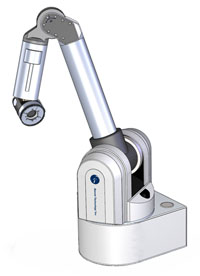
\includegraphics[height=4cm]{Img/set_up/wam.jpg}
\caption{Barrett WAM arm}\label{fig:wam_1}
\end{subfigure}
\begin{subfigure}[b]{0.45\textwidth}
\centering
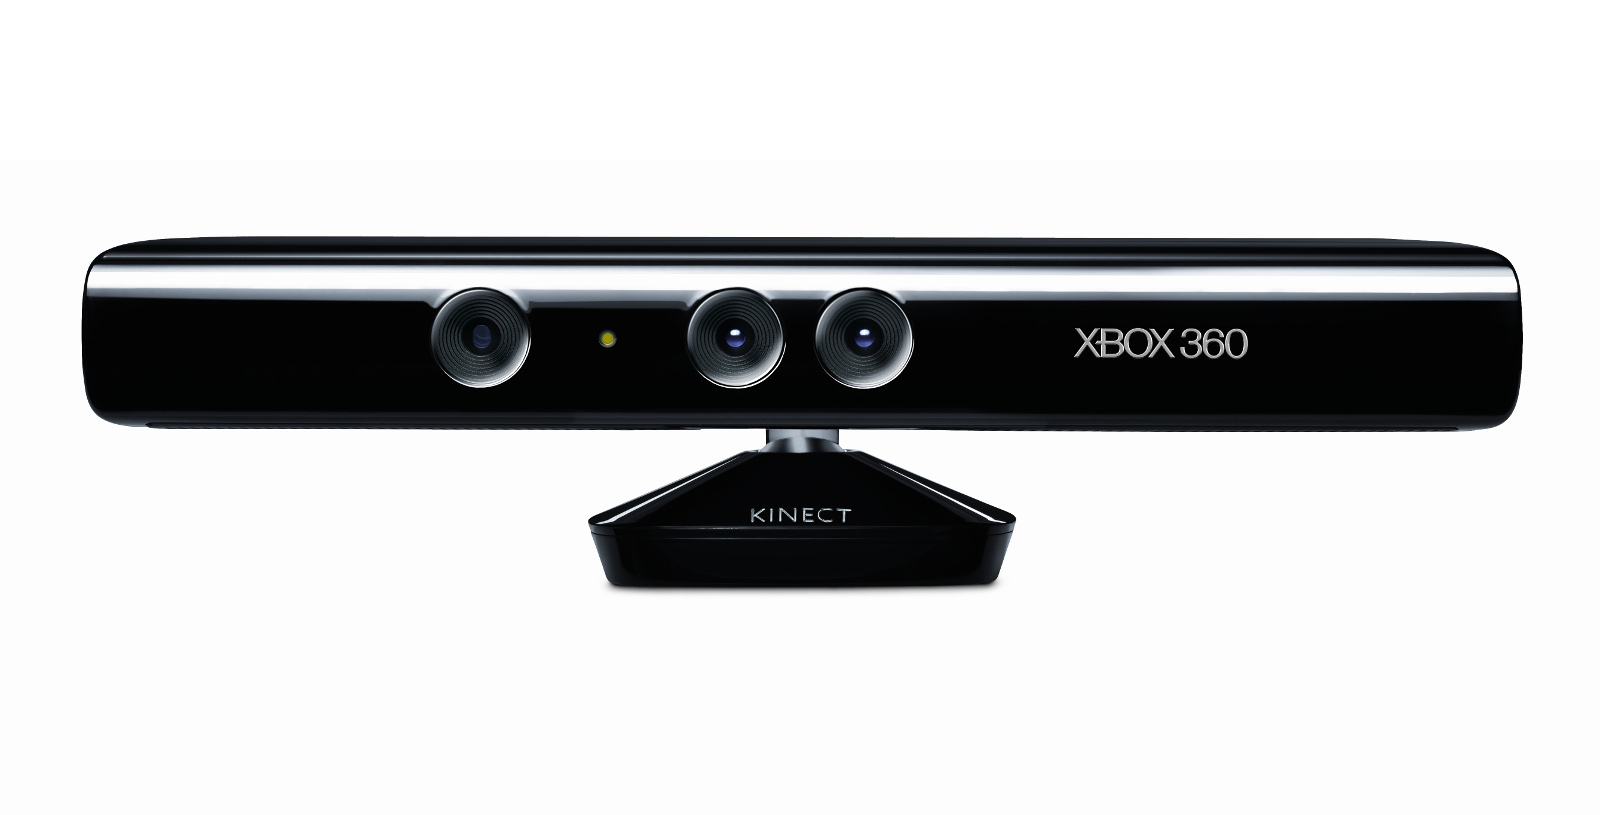
\includegraphics[width=5cm]{Img/set_up/Kinect.jpg}
\caption{Microsoft Kinect sensor}\label{fig:kinect}
\end{subfigure}
\caption{Robot and vision sensor.}
\end{figure}
%This robot is characterized by a low inertia of the end effector thanks to the kind of its actuators. 
The WAM is noteworthy because it does not use any gears for manipulating the joints, but cable drives, so there are no backlash problems and it is both fast and stiff. Cable drives permit low friction and ripple-free torque transmission from the actuator to the joints. 
To detect the objects a Kinect camera, a RGB-D sensor, is employed (\figref{fig:kinect}).

To manipulate the objects the manipulation skills of the robot are enhanced by a gripper designed in the IRI institute and actuated by Dynamixel motors. Such a gripper is depicted in Figure \ref{fig:gripper_general} from several point of views. Its closing width\footnote{Distance between the fingers when the gripper is closed.} is $3$ centimetres while the opening width\footnote{Distance between the fingers when the gripper is open.} is of $8$ centimetres, therefore we are constrained to grasp objects with a width in the range $[3 \div 8]cm$.

\begin{figure}[htp]
\centering
\begin{subfigure}[b]{0.3\textwidth}
\centering
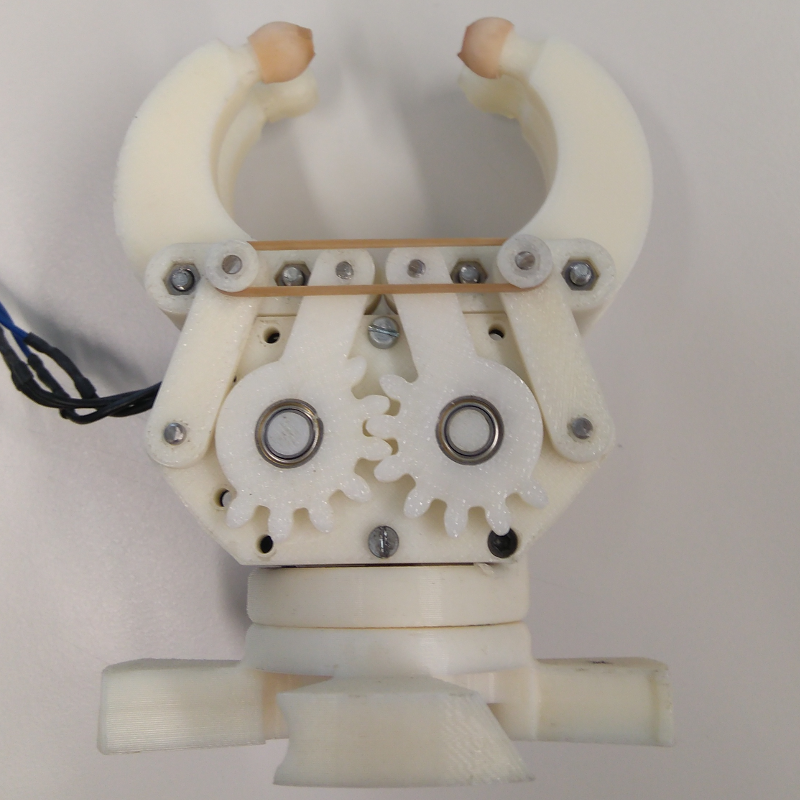
\includegraphics[height=3cm]{Img/set_up/gripper1.png}
%\caption{}
\end{subfigure}
\begin{subfigure}[b]{0.3\textwidth}
\centering
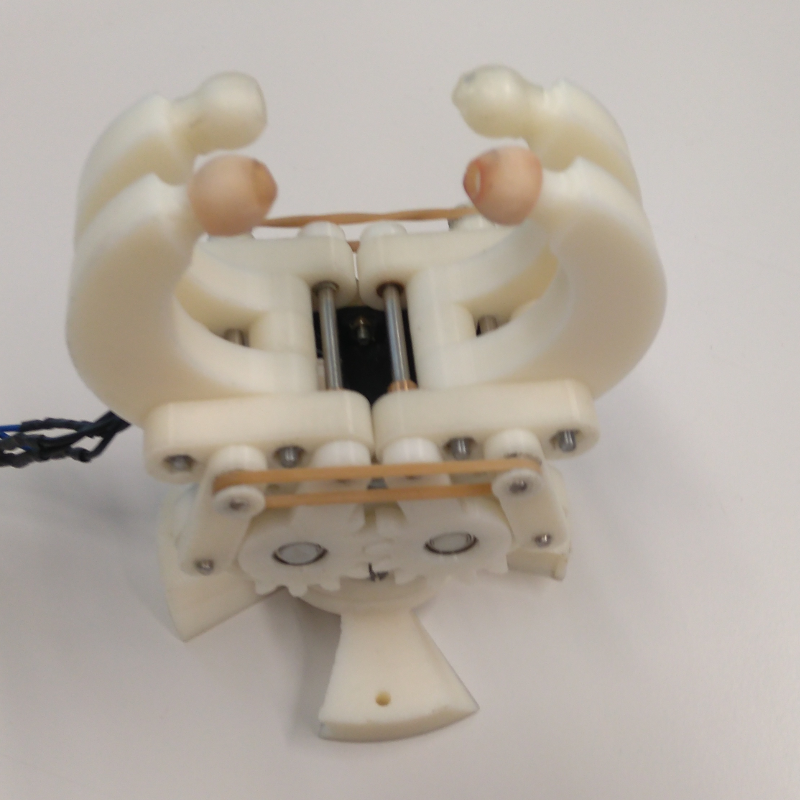
\includegraphics[height=3cm]{Img/set_up/gripper2.png}
%\caption{}
\end{subfigure}
\begin{subfigure}[b]{0.3\textwidth}
\centering
\includegraphics[width=3cm]{Img/set_up/gripper3.png}
%\caption{}
\end{subfigure}
\caption{Gripper used for the experiments}\label{fig:gripper_general}
\end{figure}

For the task planner, as the reader will see in Chapters \ref{ch:task_planner} and \ref{ch:algorithm}, the model of the gripper will be an important resource 
in order to compute the predicates. 

The gripper will be modelled measuring some principal elements such as: finger's width and height, gripper's width, height and deep, closing and opening width. The modelling procedure is depicted in Figure \ref{fig:gripper_modelling}. The resulting model is a simple triangle mesh which includes all the important geometric information of the gripper.
\begin{figure}[h]
\centering
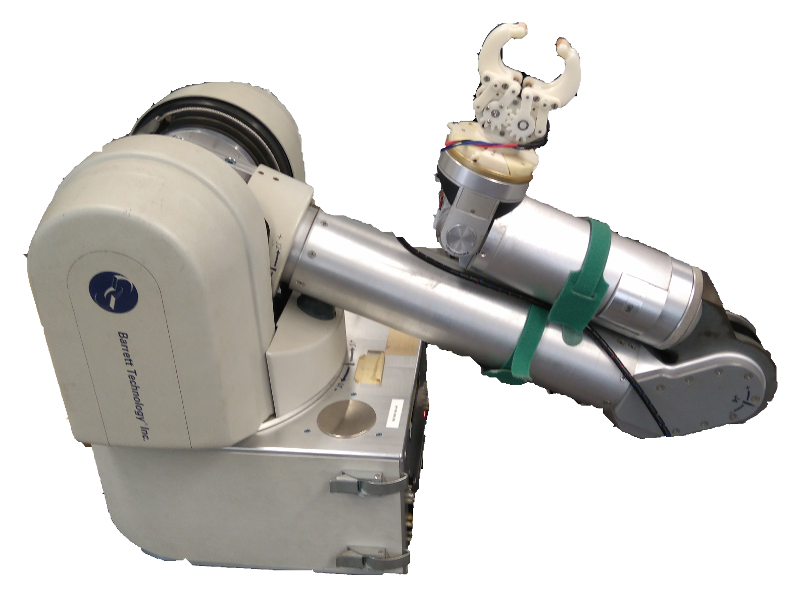
\includegraphics[width=5.0cm]{Img/set_up/wam_gripper2.png}
\caption{Gripper and WAM.}\label{fig:wam_gripper}
\end{figure}
Such a simple model allows the collision algorithm commented in Chapter \ref{ch:algorithm} to check for collision in just few millisecond. 
A more detailed and complex model would only lead as benefit a higher precision, but for this kind of task an extremely accurate precision is not needed, and it will slow down the algorithm because the collision checking procedure would be more computationally expensive. 
The gripper will be mounted in the end effector of the robot as shown in Figure \ref{fig:wam_gripper}. 


\begin{figure}[htp]
\centering
\begin{subfigure}[t]{0.25\textwidth}
\centering
\stackunder[5pt]	{\includegraphics[height=3cm]{Img/set_up/gripper_modelling1.png}}{Elements measured}
\end{subfigure} 
\begin{subfigure}[t]{0.3\textwidth}
\centering
\stackunder[5pt]	{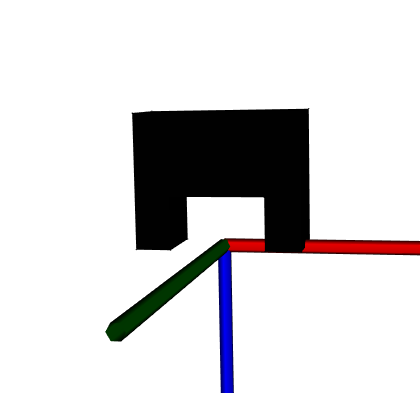
\includegraphics[height=3cm]{Img/set_up/gripper_open_model.png}}{Opened gripper mesh model}
\end{subfigure}
\hspace{1cm}
\begin{subfigure}[t]{0.3\textwidth}
\centering
\stackunder[5pt]	{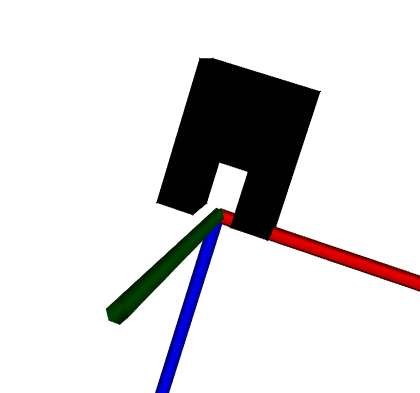
\includegraphics[height=3cm]{Img/set_up/gripper_closed_model.png}}{Closed gripper mesh model}
%\caption{}
\end{subfigure}
\caption{At the left the principal elements measured are highlighted for the opened gripper model. The gripper mesh model is here shown in the PCL visualizer. The \textcolor{red}{red}, \textcolor{green}{green} and \textcolor{blue}{blue} axis are respectively the x, y and z axis. }\label{fig:gripper_modelling}
\end{figure}

The scenario the robot is going to work in is composed of a table and the objects will lay on top of it. In Figure \ref{fig:setup_} the main elements of the set up are highlighted. The WAM arm's base is in a fixed position with respect the table and the Kinect camera is located on top of the table pointing down. The Kinect is calibrated and the fixed transformation between the Kinect's frames and the base frame of the robot is known, so all the points measured by the Kinect can be expressed in coordinates with respect the robot's base frame. An example of a cluttered scene the robot is going to deal with in this thesis is depicted in Figure \ref{fig:example_scene}, and the same scene seen by the Kinect is shown in Figure \ref{fig:kinect_view}. With respect the kinect's view the robot is located at the top side of the image, outside the field of view of the Kinect, in order to avoid to detect the arm as an object. If the robot arm would be present in the depth image we should apply some algorithms to identify the robot arm, which could also produce important occlusions, that is hide some objects from the Kinect's view. In order to avoid all this, the depth images considered are the ones provided by the Kinect when the robot is no more in the Kinect's view (these poses are known a priori). 

\begin{figure}[htp]
\centering
\begin{subfigure}[b]{0.4\textwidth}
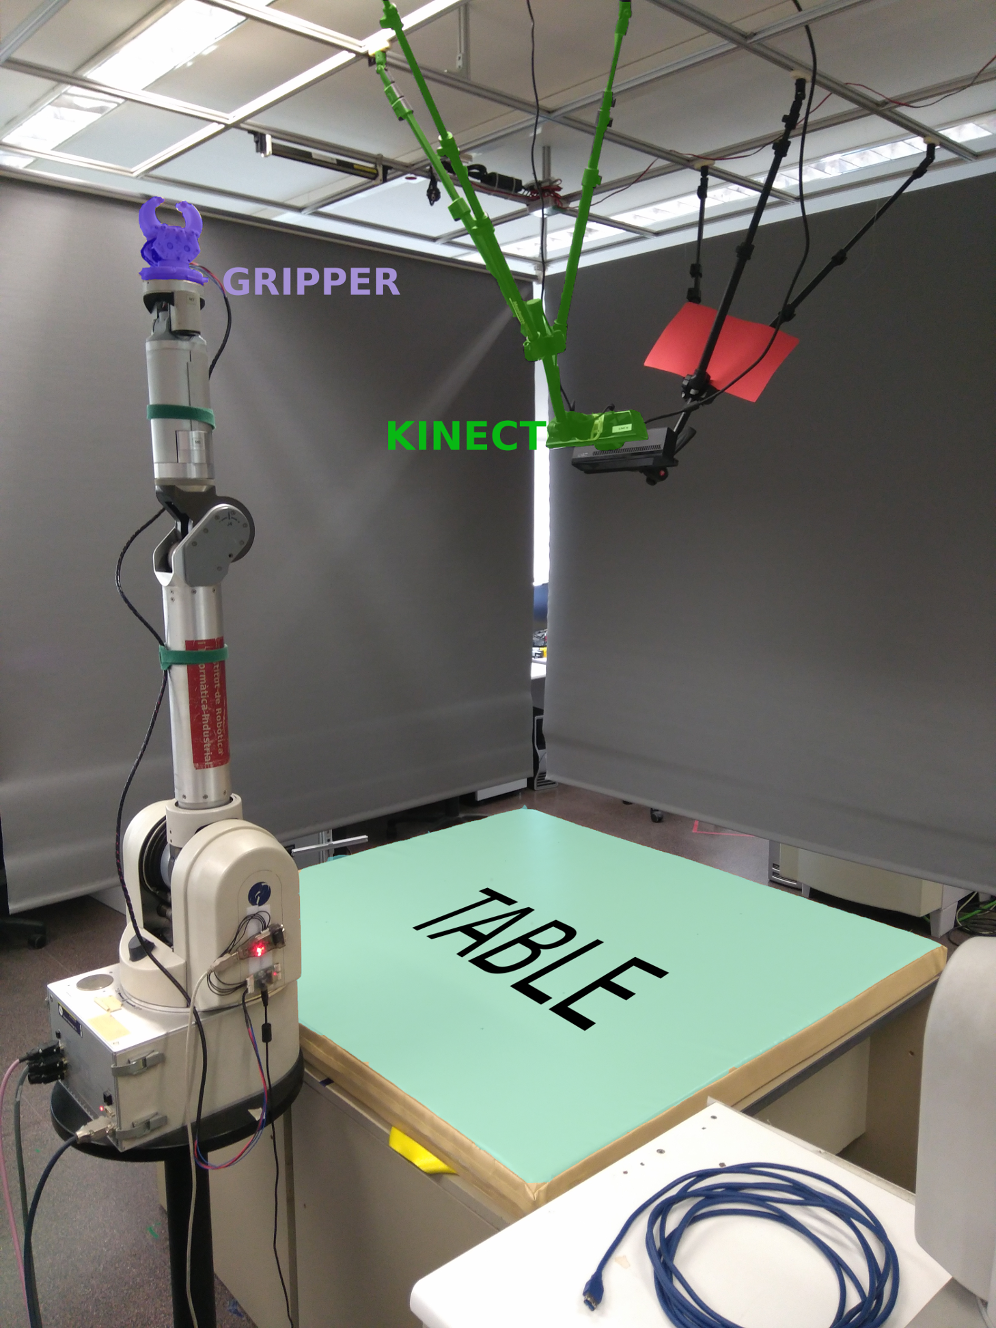
\includegraphics[height=7.5cm]{Img/set_up/set_up_nice2.png}
\caption{Principal elements of the experimental set up.}\label{fig:setup_}
\end{subfigure}
\qquad \qquad 
\begin{subfigure}[b]{0.4\textwidth}
\centering
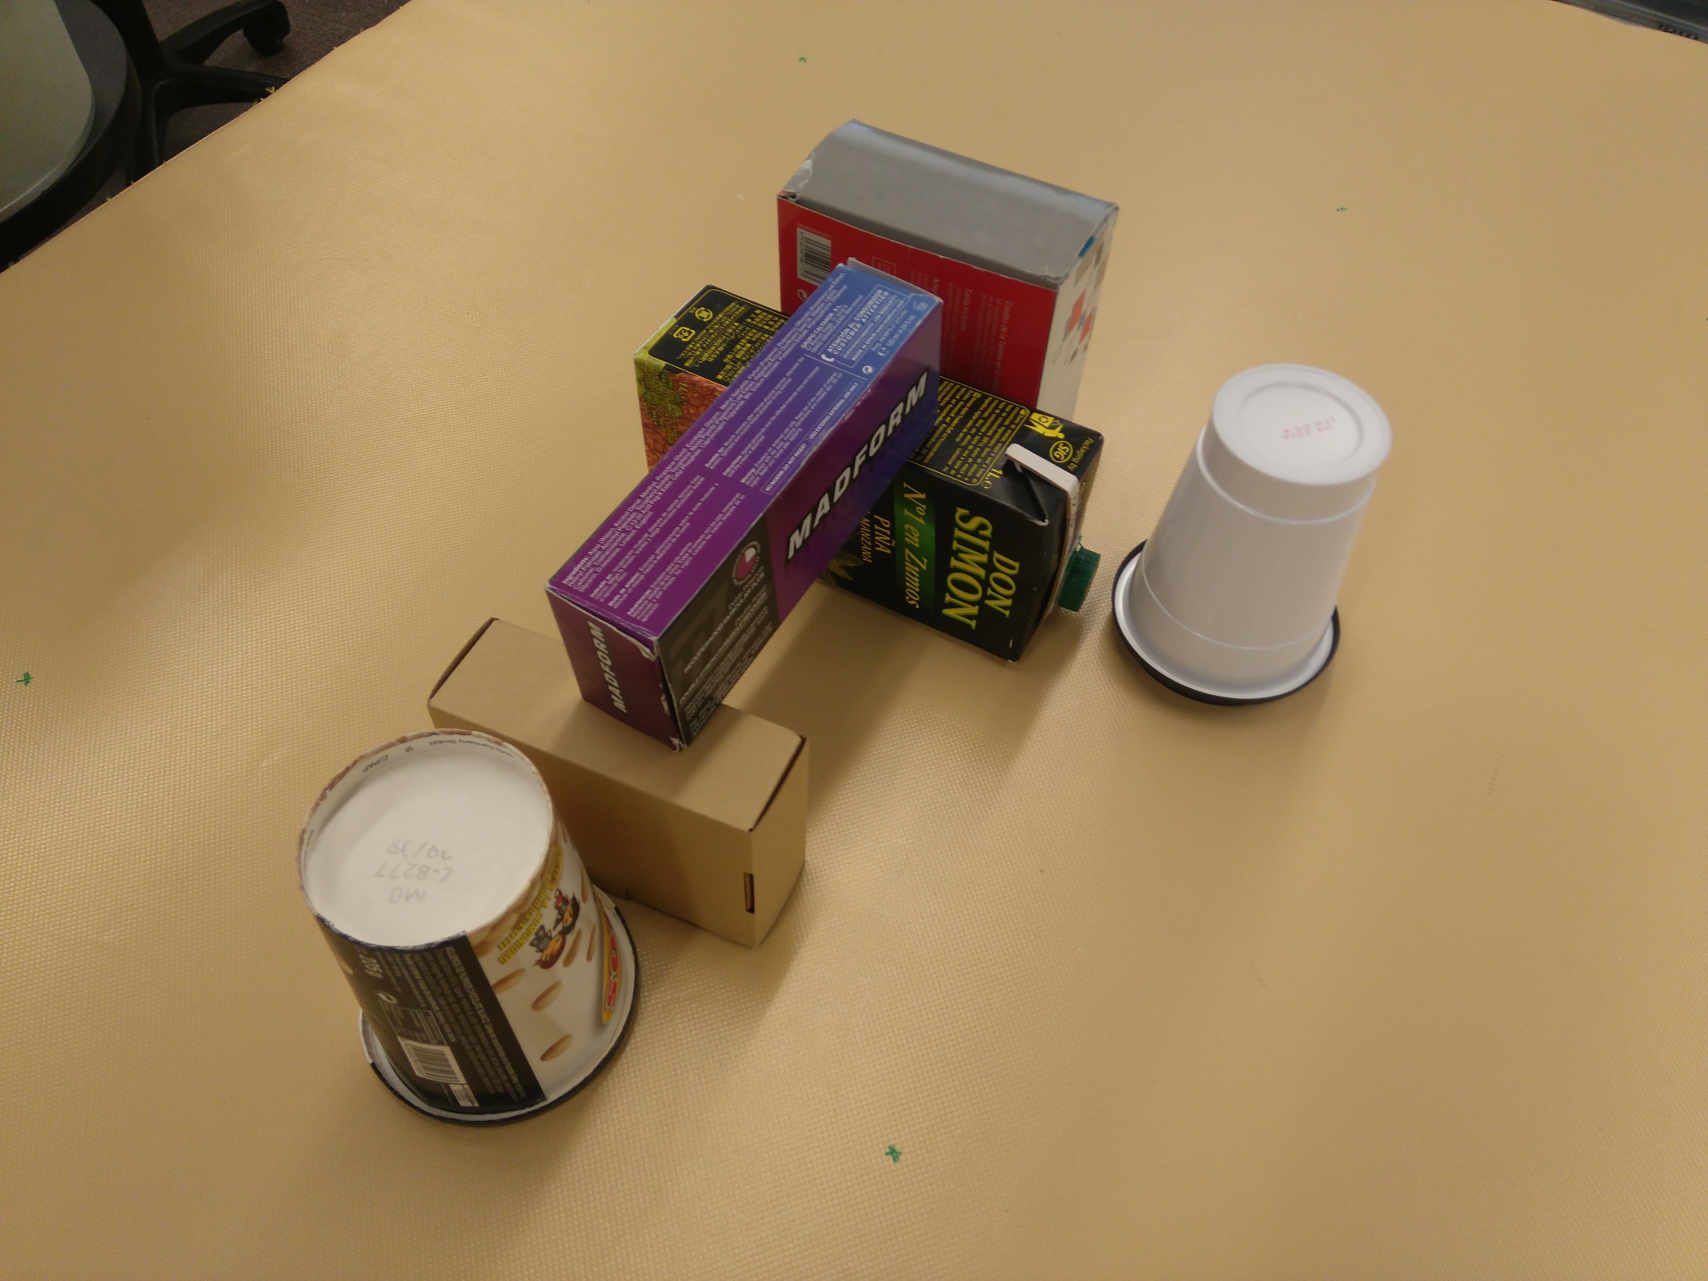
\includegraphics[height=3cm]{Img/set_up/example_setup.jpg}
\caption{Example of a cluttered scene the robot is going to work with.}\label{fig:example_scene}
\vspace{2ex}
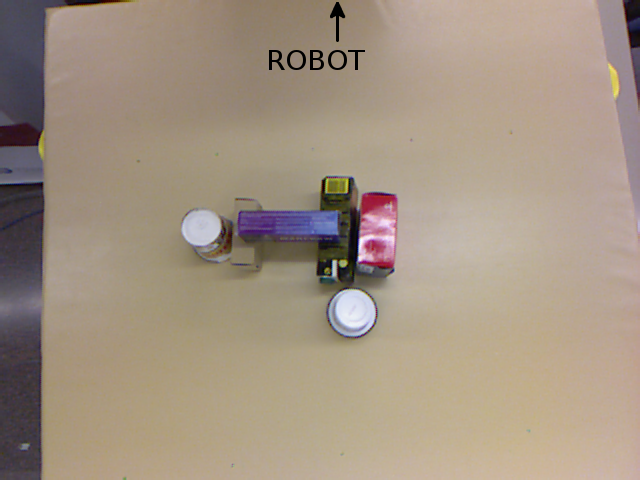
\includegraphics[height=3cm]{Img/set_up/view_kinect.png}
\caption{Kinect's view.}\label{fig:kinect_view}
\end{subfigure}
\caption{Experimental set up, and an example of a cluttered scene the robot is going to interact with.}
\label{fig:setup}
\end{figure}


%Concerning the example of Figure \ref{fig:example_scene} it can be appreciated that the manipulation needed in order to clean all the table with carefulness is quite complex. All the sequence of actions will be retrieved by the planner.



